\chapter{Results and Observations}
\label{ch:SC}

\paragraph{}
The KNN Classifier was tested with the value of k = 1 to reduce the number of computations as much as possible to speed up the process. All decision tree based classifiers have been tested with max\_depth = 2 and 4. This parameter defines how deep the tree can build itself. In the case of DecisionTreeClassifier, max\_depth = None has also been considered. The execution time and accuracy for each model is presented in Table \ref{res_all} and Table \ref{res_2}

\begin{table}[h]
    \caption{Execution times of different models with all features}
    \centering
    \label{res_all}
    \begin{tabular}{| l | r | r | r |}
        \hline
        \textbf{Model} & \textbf{TTF (sec)} & \textbf{TTP (sec)} & \textbf{Accuracy} \\
        \hline
        KNeighborsClassifier(n\_neighbors = 1) & 78.721 & 54.251 & 0.9519 \\
        \hline
        GaussianNB() & 0.752 & 0.77 & 0.9181 \\
        \hline
        DecisionTreeClassifier() & 3.76 & 0.3 & 0.9746 \\
        \hline
        DecisionTreeClassifier(max\_depth = 2) & 3.463 & 0.295 & 0.9873 \\
        \hline
        DecisionTreeClassifier(max\_depth = 4) & 3.781 & 0.32 & 0.9876 \\
        \hline
        RandomForestClassifier(max\_depth = 2) & 4.666 & 0.472 & 0.9885 \\
        \hline
        RandomForestClassifier(max\_depth = 4) & 7.144 & 0.521 & 0.99 \\
        \hline
        ExtraTreesClassifier(max\_depth = 2) & 1.167 & 0.489 & 0.9276 \\
        \hline
        ExtraTreesClassifier(max\_depth = 4) & 1.604 & 0.551 & 0.9617 \\
        \hline
    \end{tabular}
\end{table}

\begin{table}[h]
    \caption{Execution times of different models with 2 selected features}
    \centering
    \label{res_2}
    \begin{tabular}{| l | r | r | r |}
        \hline
        \textbf{Model} & \textbf{TTF (sec)} & \textbf{TTP (sec)} & \textbf{Accuracy} \\
        \hline
        KNeighborsClassifier(n\_neighbors = 1) & 0.909 & 0.192 & 0.9895 \\
        \hline
        GaussianNB() & 0.073 & 0.039 & 0.9860 \\
        \hline
        DecisionTreeClassifier() & 0.057 & 0.013 & 0.9895 \\
        \hline
        DecisionTreeClassifier(max\_depth = 2) & 0.075 & 0.023 & 0.98733 \\
        \hline
        DecisionTreeClassifier(max\_depth = 4) & 0.195 & 0.013 & 0.9895 \\
        \hline
        RandomForestClassifier(max\_depth = 2) & 0.902 & 0.192 & 0.9885 \\
        \hline
        RandomForestClassifier(max\_depth = 4) & 1.027 & 0.219 & 0.9895 \\
        \hline
        ExtraTreesClassifier(max\_depth = 2) & 0.55 & 0.198 & 0.9826 \\
        \hline
        ExtraTreesClassifier(max\_depth = 4) & 0.654 & 0.221 & 0.9895 \\
        \hline
    \end{tabular}
\end{table}

\paragraph{}
To understand the difference in the performance of these models, a better visualization of the data in Table \ref{res_all} and Table \ref{res_2} is presented in Figure \ref{ttf_improvement}, Figure \ref{ttp_improvement} and Figure \ref{acc_improvement}.

\begin{figure}[h]
    \hfill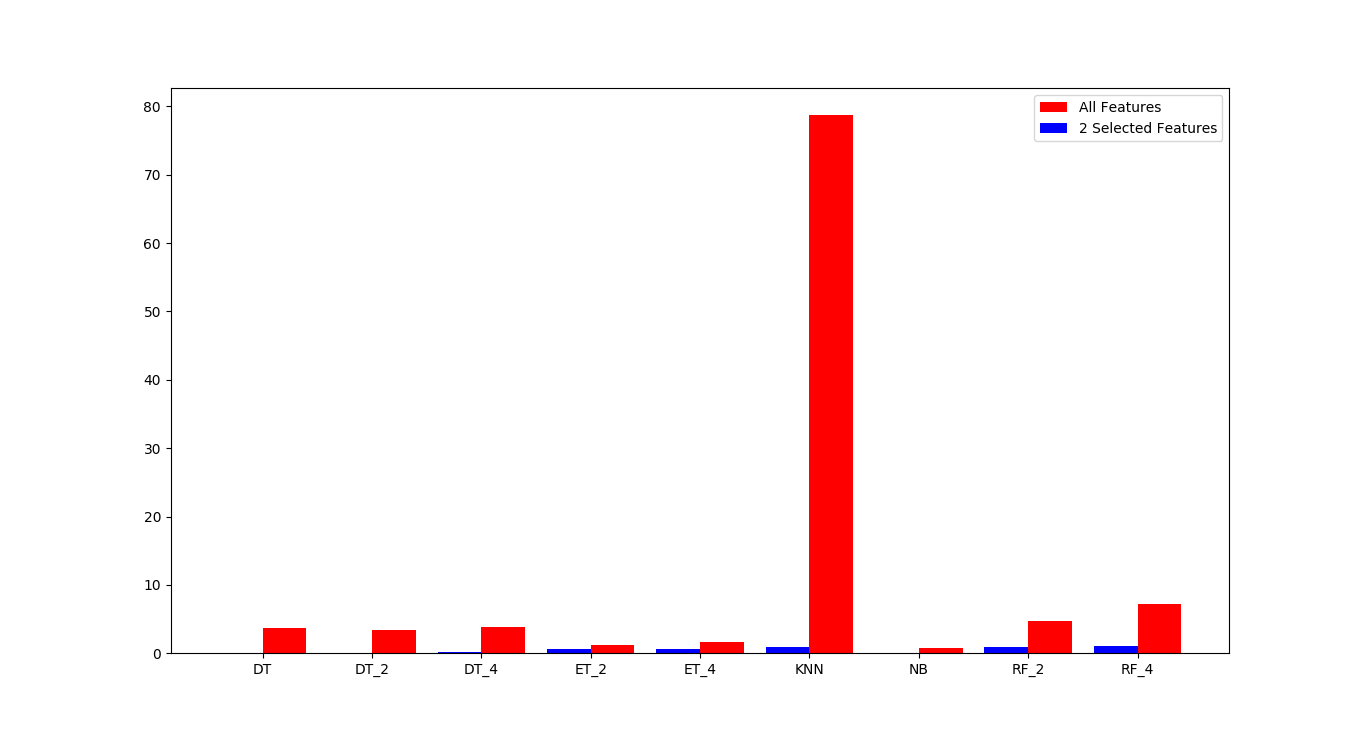
\includegraphics[width=1\textwidth]{Chapter4/ttf_improvement}\hspace*{\fill}
    \caption{Change in TTF of different models (lower is better)}
    \label{ttf_improvement}
\end{figure}

\begin{figure}[h]
    \hfill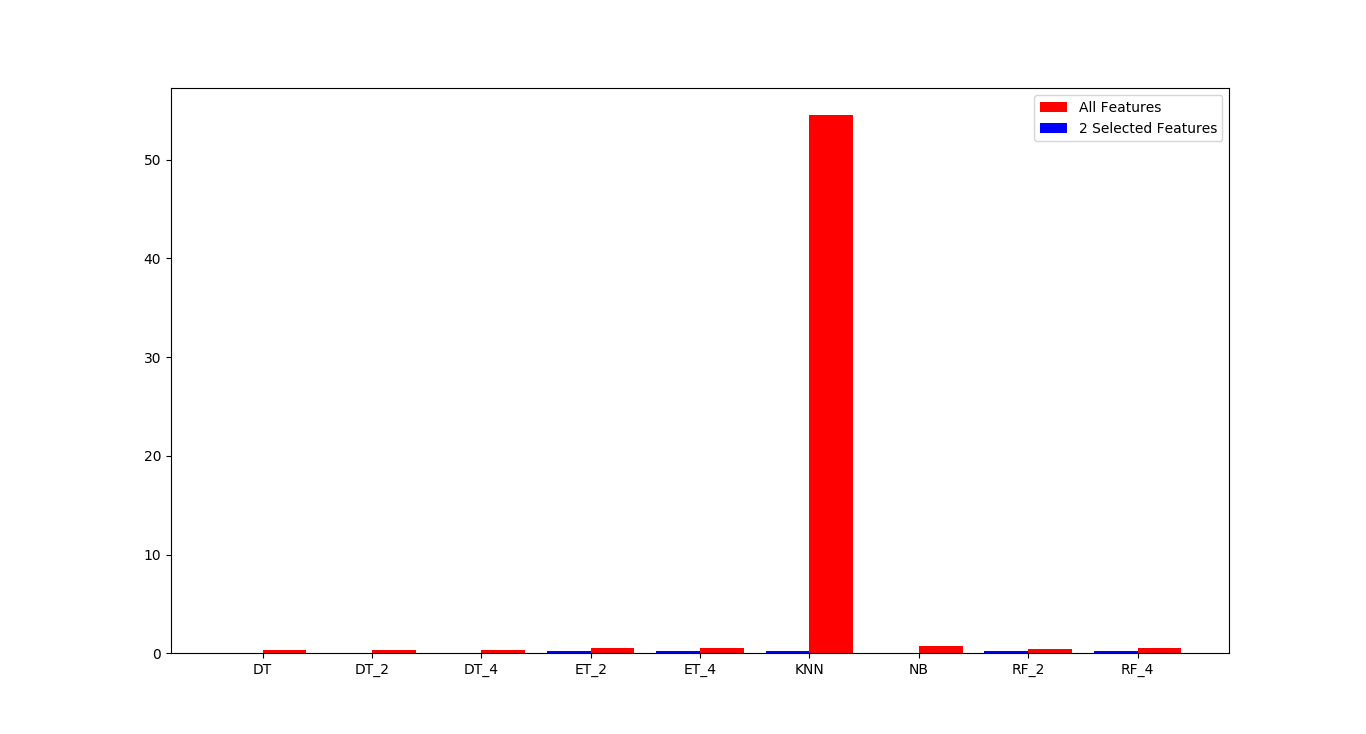
\includegraphics[width=1\textwidth]{Chapter4/ttp_improvement}\hspace*{\fill}
    \caption{Change in TTP of different models (lower is better)}
    \label{ttp_improvement}
\end{figure}

\begin{figure}[h]
    \hfill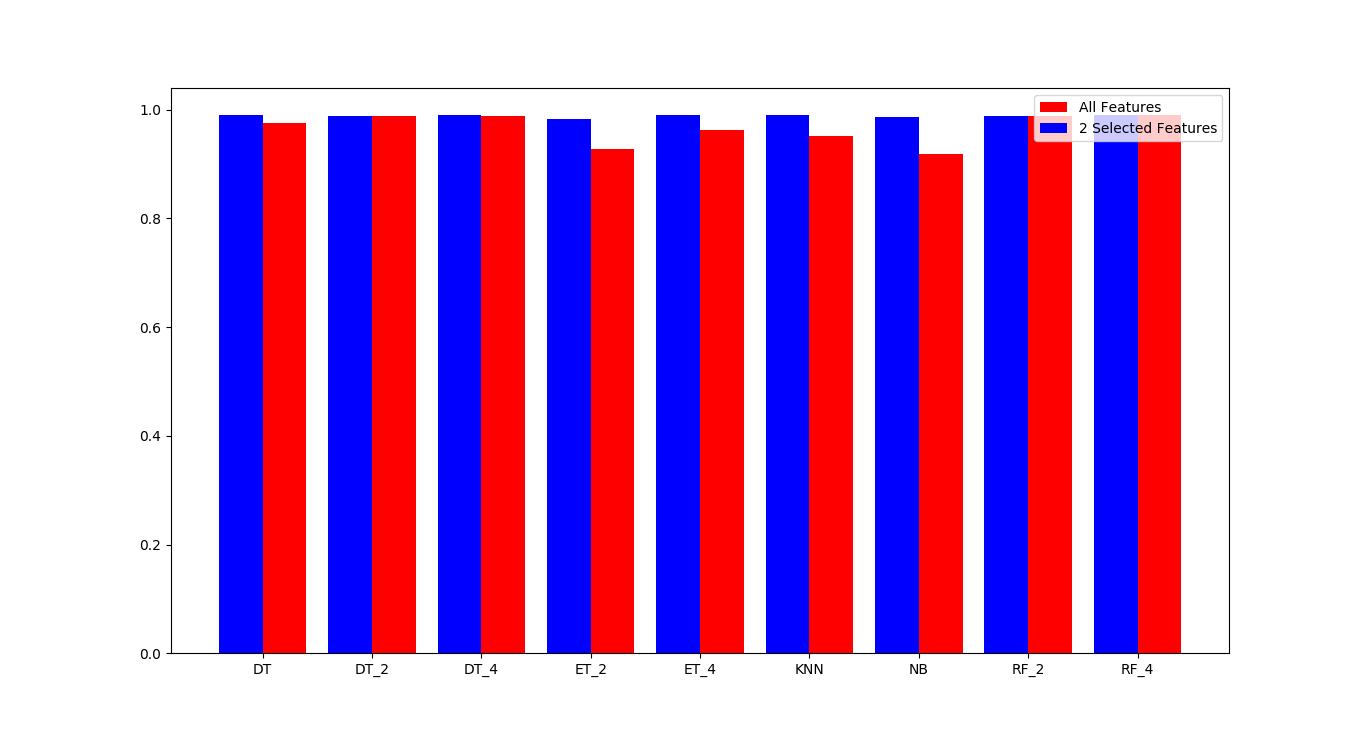
\includegraphics[width=1\textwidth]{Chapter4/acc_improvement}\hspace*{\fill}
    \caption{Change in Accuracy of different models (higher is better)}
    \label{acc_improvement}
\end{figure}

\paragraph{}
It is clear from these results that selecting the 2 features mentioned in Section \ref{feature_select} resulted in radically reduced execution times, especially for KNN (77.812 seconds reduced), without negatively affecting to the accuracy of the models. Most models see only slight change in accuracy, but the change itself is usually positive. The reduction in execution time resulted in significant improvement in the Training and Prediction Scores (Table \ref{final_scores}).

\begin{table}
    \caption{Training and Prediction Scores}
    \label{final_scores}
    \begin{tabular}{| l | r | r | r | r |}
        \hline
         & \multicolumn{2}{c |}{\textbf{All Features}} & \multicolumn{2}{c |}{\textbf{2 Features}} \\
        \hline
        \textbf{Model} & \textbf{TS} & \textbf{PS} & \textbf{TS} & \textbf{PS} \\
        \hline
        KNeighborsClassifier(n\_neighbors = 1) & 0.012 & 0.017 & 1.088 & 5.153 \\
        \hline
        GaussianNB() & 1.22 & 1.192 & 13.507 & 25.282 \\
        \hline
        DecisionTreeClassifier() & 0.259 & 3.248 & 17.359 & 76.115 \\
        \hline
        DecisionTreeClassifier(max\_depth = 2) & 0.285 & 3.346 & 13.164 & 42.927 \\
        \hline
        DecisionTreeClassifier(max\_depth = 4) & 0.261 & 3.086 & 5.074 & 76.115 \\
        \hline
        RandomForestClassifier(max\_depth = 2) & 0.211 & 2.094 & 1.095 & 5.148 \\
        \hline
        RandomForestClassifier(max\_depth = 4) & 0.138 & 1.9 & 0.963 & 4.518 \\
        \hline
        ExtraTreesClassifier(max\_depth = 2) & 0.794 & 1.896 & 1.786 & 4.962 \\
        \hline
        ExtraTreesClassifier(max\_depth = 4) & 0.599 & 1.745 & 1.513 & 4.477 \\
        \hline
    \end{tabular}
\end{table}

\begin{table}
    \caption{Confusion Matrix for the models}
    \centering
    \label{confusion_matrix}
    \begin{tabular}{| l | r | r | r | r |}
        \hline
        \textbf{Model} & \textbf{TN} & \textbf{FN} & \textbf{FP} & \textbf{TP} \\
        \hline
        KNN & 639191 & 25586 & 8060 & 27163 \\
        \hline
        KNN & 640364 & 463 & 6887 & 52286 \\
        \hline
        NB & 641671 & 51709 & 5580 & 1040 \\
        \hline
        NB & 637461 & 0 & 9790 & 52749 \\
        \hline
        DT & 642239 & 12715 & 5012 & 40034 \\
        \hline
        DT & 640364 & 462 & 6887 & 52287 \\
        \hline
        DT\_2 & 638630 & 248 & 8621 & 52501 \\
        \hline
        DT\_2 & 638630 & 248 & 8621 & 52501 \\
        \hline
        DT\_4 & 638740 & 146 & 8511 & 52603 \\
        \hline
        DT\_4 & 640364 & 463 & 6887 & 52286 \\
        \hline
        RF\_2 & 639520 & 278 & 7731 & 52471 \\
        \hline
        RF\_2 & 639537 & 284 & 7714 & 52465 \\
        \hline
        RF\_4 & 642116 & 1837 & 5135 & 50912 \\
        \hline
        RF\_4 & 640364 & 463 & 6887 & 52286 \\
        \hline
        ET\_2 & 645241 & 48667 & 2010 & 4082 \\
        \hline
        ET\_2 & 639942 & 4829 & 7309 & 47920 \\
        \hline
        ET\_4 & 644140 & 23672 & 3111 & 29077 \\
        \hline
        ET\_4 & 640371 & 468 & 6880 & 52281 \\
        \hline
    \end{tabular}
\end{table}

\paragraph{}
The data in Table \ref{final_scores} is presented in Figure \ref{ps_improvement} and Figure \ref{ts_improvement} for visualizing the change in the Training and Prediction Scores. It is evident from these results that the two selected features in the dataset are indeed contributing the most in the classification. Accuracy and execution time improved upon ignoring the other features. The time reduction is because there are less dimensions in the feature space for the models to process, while the accuracy improvement may suggest that the other features had a slight negative contribution in the classification. A closer look at the confusion matrix results (Table \ref{confusion_matrix}) suggests that, although the overall accuracy has improved, the false positive rate in most cases has increased.

\begin{figure}[h]
    \hfill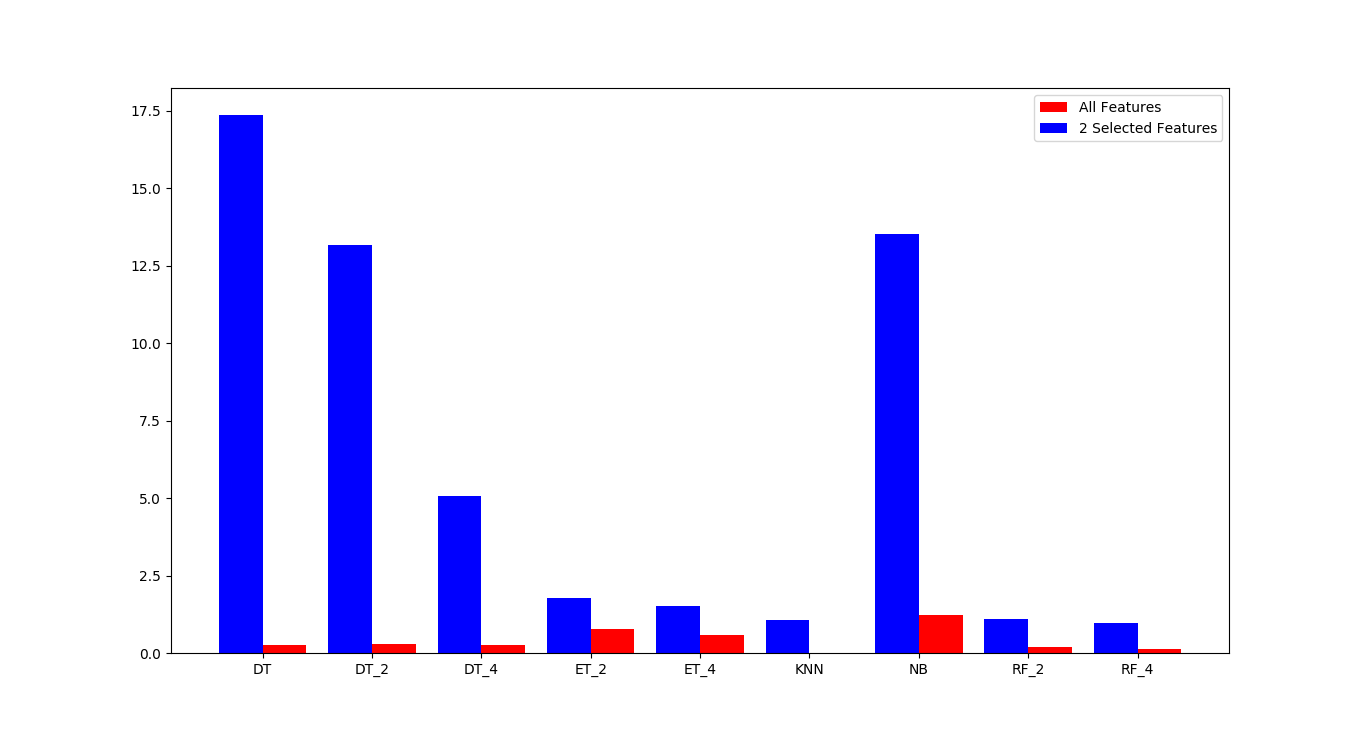
\includegraphics[width=1\textwidth]{Chapter4/ts_improvement}\hspace*{\fill}
    \caption{Change in TS of different models (higher is better)}
    \label{ts_improvement}
\end{figure}

\begin{figure}[h]
    \hfill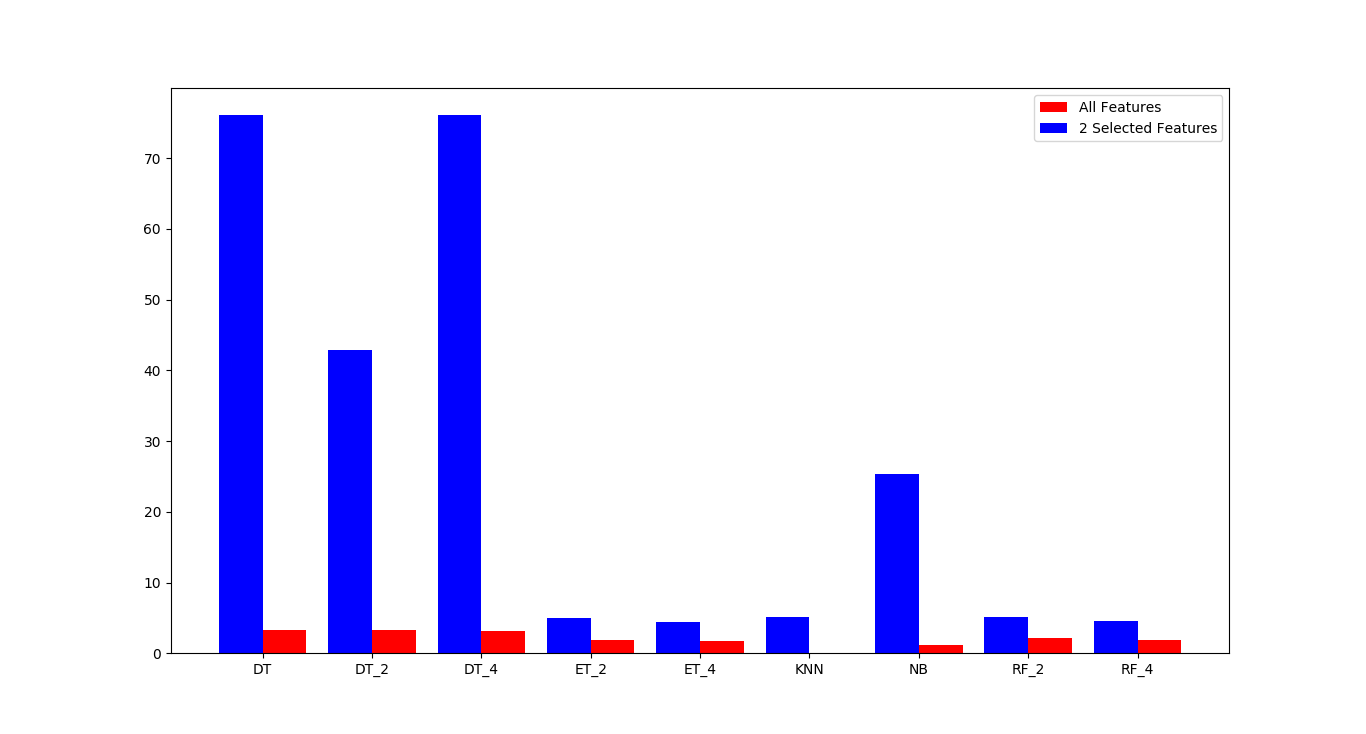
\includegraphics[width=1\textwidth]{Chapter4/ps_improvement}\hspace*{\fill}
    \caption{Change in PS of different models (higher is better)}
    \label{ps_improvement}
\end{figure}
